%!TEX root = thesis.tex





%
%==========================================================================================
%
\chapter{Combining Time Scales and Modalities}
\label{chap:combine}

Each human tends to perform activities in a specific way, be it on the micro or macro scale. However, the behavior of the persons in our system is actually monitored from three different points of view. In the first of these, denoted as the \textit{micro level}, one typically deals with behavior that changes in tenths of a second or seconds. For example, one person always carries his identity card in a wallet and puts the whole wallet near the wireless identity-card reader, while another person carries her card in a handbag and requires some time to take it out, identify herself, and put the card back. The person's movement around the access point depends on his/her habits and mental/physical state. These facts determine the persons' patterns at the micro level.

The second viewpoint, denoted as the \textit{macro level}, describes the persons' daily routines. The activities of interest are the arrival times at access points, the movements between various access points in the access-control network, and even the connections between persons, for example, person $A$ often enters a short time after person $B$. The time scale used at the macro level can vary from seconds to months.

The third viewpoint, denoted as the \textit{visual level}, captures the persons' visual movement at an access point using a camera. It is also focused on micro-level movements; that is, behavior that changes over a short time interval, but in addition to micro-level features, it obtains features from the visual characteristics of the person and his/her movement, for example, the person's height and the door-opening dynamics.

Several rules additionally control the regular entry procedure, the regular working time, and the access permissions.


%\section{Time Scales}
%\section{Modalities}

\section{A Bayesian Network Model}

After the expert rules, micro, macro, visual and meta-learning have made their assessments, their results are integrated into a joint risk analysis of the current entry. It estimates the probability of the event $E = $ \textit{entry is regular} given the observations of the modules. If the estimated probability does not exceed a threshold value, an alarm is triggered. Note that an alarm can also be triggered by expert rules when there is sufficient certainty (type 1 rules).

The reasoning in the prototype system is performed with a Bayesian network, structured as shown in Figure~\ref{fig:bayesianNetwork}. Four modules have a direct impact on the event $E$; that is, expert rules, micro learning and visual learning, and a macro meta-learning module, while the macro meta-learning module depends only on the three macro modules. The probabilities in the network are computed from the test data, using the \textit{m-estimate}  for conditional probabilities and the \textit{Laplace estimate} for a-priori probabilities. 
\begin{figure}[h]
\centering
\includegraphics[bb=0 540 440 800,width=8cm]{eswa/BayesNetwork2}
%\includegraphics[bb=30 590 360 820,width=8cm]{img/BayesNetwork.pdf}
%\includegraphics[bb=0 540 440 800,width=8cm]{img/BayesNetwork2.pdf}
\caption{Bayesian network used for the reasoning.}
\label{fig:bayesianNetwork}
\end{figure}

The integration proceeds in three steps. Firstly, the output from each module is converted to interval the $[0, 1]$ representing the a-posterior probability $p_{M_i}$ that the entry is regular. Secondly, given the Bayesian network $N$ and the probabilities $p_{M_i}$, the estimated  probability of an event $E$ is computed from the network.
%\begin{eqnarray}
%P(E | M_1, M_2, \dots, M_n) = P(E) \frac{P(M_1, M_2, \dots, M_n | E)}{P(M_1, M_2, \dots, M_n)}
%\end{eqnarray}
%Numerator is developed with chain rule and due to the structure of the network is simplified to:
%\begin{multline}
%P(M_1, M_2, \dots, M_n | E) = \prod_{i=1}^{n} P(M_i | Parents(M_i)) = \\
% = \prod_{i=1}^{n} p_{M_i} P(M_i=1|E) + (1-p_{M_i}) P(M_i=0|E)
%\end{multline}
%Denominator, on the other hand, is independent of the event E, thus is developed as follows:
%\begin{multline}
%P(M_1, M_2, \dots, M_n) = \\
% = \sum_{e\in\{0, 1\}} P(E=e) P(M_1, M_2, \dots, M_n | E=e)  =\\
% = \sum_{e\in\{0, 1\}} P(E=e) \prod_{i=1}^{n} (p_{M_i} P(M_i=1|E=e) + \\
% + (1-p_{M_i}) P(M_i=0|E=e))
%\end{multline}

Finally, the integration module outputs the joint analysis as a probability that the entry is regular and provides an explanation. According to the threshold values, the integration module triggers \textit{alarm} or \textit{OK} and stores the results in the ontology. In high-security areas, the cost of a false alarm is negligible compared to the cost of an unrecognized intruder; therefore, the system is set to minimize the latter.


